
% JuliaCon proceedings template
\documentclass{juliacon}
\setcounter{page}{1}

\usepackage{amsmath}
%\usepackage[ruled,vlined]{algorithm2e}
%\usepackage{algorithm, algorithmic}

\usepackage{booktabs}
\usepackage[width=.45\textwidth]{caption}

\usepackage{graphicx}
\graphicspath{{../figures/}}

\begin{document}

% **************GENERATED FILE, DO NOT EDIT**************

\title{Julia for HPC: In Situ data Analysis with Julia for Climate Simulations at Large Scale}



\author[1]{Li Tang}
\author[2]{Soumya Dutta}
\author[1]{Natalie Klein}
\author[3]{Wayne Yu Wang}
\author[1]{Jonathan David Wolfe}
\author[1]{Luke Van Roekel}
\author[4]{Nathan Urban}
\author[1]{Ayan Biswas}
\author[1]{Earl Lawrence}
\affil[1]{Computer, Computational, and Statistical Sciences (CCS), Los Alamos National Laboratory}
\affil[2]{Department of Computer Science and Engineering, Indian Institute of Technology Kanpur}
\affil[3]{Department of Statistics, University of Michigan}
\affil[4]{Computational Science Initiative, Brookhaven National Laboratory}



\keywords{Julia, High-performance computing, In Situ data analysis, Scientific computing, Climate simulations, E3SM}

\hypersetup{
pdftitle = {In-Situ E3SM},
pdfsubject = {JuliaCon 2022 Proceedings},
pdfauthor = {1st author, 2nd author, 3rd author},
pdfkeywords = {Julia, In-Situ data analysis, Scientific computing, Climate simulations},
}



\maketitle

\begin{abstract}

Fast-evolving data science techniques have enabled scientific discoveries in part by providing the ability to analyze large amounts of scientific data and extract relevant patterns.  Scientific simulations offer a unique opportunity to study large-scale, complex systems, such as the Earth's climate, under varying conditions and modeling assumptions. However, one major obstacle to improved utilization of large scientific simulations is the ever-increasing gap between computing speed, which continues to increase, and data I/O bandwidth, which remains relatively constant. This mismatch often prevents full utilization of the data; we are likely unable to save all of the generated data for analysis, and simple solutions such as saving compressed versions of the data for later analysis may be insufficient to answer questions of interest.

In situ data analysis techniques seek to address this issue by completing analysis and pattern extraction from generated scientific data while the application is running, and the in situ data analysis only involves compute and in-memory data I/O, which improves performance. However, one major challenge of employing in situ data analysis to legacy scientific applications is that modern advanced data science techniques are usually not implemented in the same way as the scientific codes (typically, using the Fortran programming language with parallel programming models). To address this challenge, we develop an infrastructure for coupling a popular high-level data science programming language, Julia, with the large-scale production-level climate code Energy Exascale Earth System Model (E3SM) on high performance computing (HPC) systems. To demonstrate the infrastructure, we develop two in situ data analysis methods in Julia and evaluate their performance and the infrastructure overhead. Our results show that our in situ Julia data analysis methods are able to detect extreme weather events and characterize climate patterns with insignificant infrastructure overhead. Furthermore, our infrastructure allows user-friendly development and deployment of new Julia data analysis modules without the need to recompile the simulation code, giving data analysts a simple new tool for in situ analysis.

%\headingtable

\end{abstract}

\section{Introduction}

Computing devices are evolving much faster than storage devices because of their different ratios of performance improvement to R\&D investment in the post-Moore’s Law era~\cite{thompson2018decline}. This trend enlarges the performance gap between our computing and storage devices and greatly limits our ability to analyze all the generated scientific simulation data. When run on HPC systems, modern physics simulations employ thousands of nodes, generating large amounts of data. While this data could possibly be stored for post-processing, write time to disk, available storage space, and post-processing time can be prohibitive, especially at high physics simulation resolution.  At such a high resolution, the three-dimensional physics model state alone can be tens of gigabytes \emph{per} time slice. To address these issues, we adopt in situ data analysis to analyze physics simulation data as the simulation is running. 


Our target HPC application is Energy Exascale Earth System Model (E3SM)~\cite{golaz2019doe}. E3SM is the Department of Energy (DOE) state-of-the-science earth system model. It aims to address the most critical and challenging climate problems pertaining to the DOE energy and water security mission by efficiently utilizing DOE’s advanced HPC systems. E3SM includes multiple Earth system components and one coupler to incorporate the components. In this paper, we focus on E3SM's atmosphere component, EAM. To perform high performance in situ data analysis on the EAM simulations, we choose Julia as the programming language because of its superior performance for data analysis and rich support of data analysis packages. Our work aims to provide data scientists with a performant interface for developing in situ data analysis algorithms without directly interacting with complex HPC codes or relying on post-hoc analysis. However, there are three challenges in doing so. First, E3SM's EAM is written in Fortran and adopts Message Passing Interface (MPI) for large-scale parallelism~\cite{walker1996mpi}, and there are no Fortran APIs for embedding Julia into EAM. Second, one MPI rank of EAM is only able to access to its local data (e.g., velocity and temperature), and each in situ Julia data analysis instance can only access the same local data of its parent EAM MPI rank. Last, EAM is compiled and interacting with other E3SM components, and the in situ Julia data analysis should be noninvasive to other E3SM components. To address these challenges, we develop and implement an infrastructure for coupling the Julia runtime with E3SM, which enables effective transfer of data and consistent MPI communication between Julia and E3SM through a minimalist design. 



To demonstrate the in situ Julia data analysis infrastructure, we implement two in situ data analysis methods in Julia: (1) detection of Sudden Stratospheric Warming (SSW) with generalized extreme value (GEV) analysis, and (2) characterization of large-scale climate patterns via principal components analysis (PCA). SSW events are extreme events in the upper atmosphere (approximately 20km above ground level) that can cause the temperature to rise as much as 50$^o$C in only a few days.  This extreme warming can destabilize the polar vortex, which can in turn lead to rapid swings in surface air temperature. To identify SSWs, we developed an in situ analysis method that documents every occurrence when the zonal mean of the zonal wind becomes reversed (easterly) at 60°N and 10 hPa and lasts for at least 10 consecutive days in northern hemisphere winter. To characterize surface temperature changes that may result from SSWs, we fitted in situ generalized extreme value (GEV) models to the daily minimum surface temperatures at each spatial point in the continental United States (CONUS) via streaming variational inference~\cite{broderick2013streaming}. By updating two separate sets of models (one following SSWs and one not), we examined differences in extreme temperature behavior. Our second data analysis method focuses on PCA of the surface temperatures across the globe. PCA is a common statistical technique for identifying patterns in data that best explain variation in the data. Our TributaryPCA method estimates the top spatial principal component patterns in a streaming, distributed fashion~\cite{wang2021tributarypca}, whereas traditional analysis would need to save data from all spatial locations across many time steps to compute the principal components.


This paper presents a practical case study that uses Julia-based analysis in situ with a large-scale HPC application. The major benefit of this work is that it provides a reference design for coupling Julia with modern large-scale HPC applications which could be applied to other HPC applications with minimal effort.
In addition, data scientists could develop new Julia data analysis methods and insert them into the interface without recompiling the HPC code.
Another benefit of this work is an accurate and quantitative view of how the Julia infrastructure and coupling impact the original HPC application, which helps provide actionable guidance to HPC users before coupling Julia with their target HPC applications. To help HPC users adopt the in situ approach and Julia to meet their needs, this work provides the following key contributions:
\begin{enumerate}
\item We develop a novel in situ data analysis infrastructure for coupling E3SM with Julia for in situ data analysis at large-scale with high productivity.
\item We develop two in situ Julia data analysis methods for E3SM's EAM data at large-scale for identifying sudden stratospheric warmings and identifying dominant spatial patterns in temperature.
\item We evaluate the performance of this coupling infrastructure on a large-scale HPC system and study various design considerations, leading to guidelines for adopting Julia for in situ data analysis on other HPC applications.
\end{enumerate}


\section{Background and Related Work}
In this section, we describe the E3SM HPC simulation, the Julia programming language, and the general concept of in situ data analysis before discussing recent closely related work.

\subsection{E3SM}

E3SM is the new earth system model developed by DOE to answer critical DOE mission questions relating to energy and water security \emph{and} run efficiently on emerging HPC architectures.  E3SM includes components to model the atmosphere, land, rivers, ocean, and sea ice. The atmosphere component, EAM, utilizes a spectral element discretization on a cubed sphere grid.  The model uses approximately 110 km resolution in the horizontal and 72 vertical layers with variable spacing.  The model top is at 60km above ground level.  A detailed analysis of its performance is given in~\cite{xie2018understanding,zhang2019evaluation,qian2018parametric,rasch2019overview,golaz2019doe}.  EAM has a number of key features relative to its predecessor, which are described in~\cite{golaz2019doe}.  Of interest to our work is the linearized ozone photochemistry, which improves EAM simulations of the stratosphere, which is critically important for our SSW analysis.



\subsection{Julia}

Julia is a dynamically-typed programming language that is for general-purpose application development and provides many Python-like features (e.g., rich package support)~\cite{bezanson2012julia}. The first public Julia release was introduced in 2013 and it is designed to provide users with the speed of C/C++/Fortran~\cite{bezanson2017julia} while giving a convenient high-level programming environment. Julia is a built on top of a modularized compiler framework, Low Level Virtual Machine (LLVM)~\cite{lattner2004llvm}, and features a Just-In-Time (JIT) compilation engine~\cite{aycock2003brief}. Therefore, Julia is ideal for agile development of advanced data science algorithms due to its speed and effectiveness in solving computationally complex problems. In addition, Julia can couple with C/C++/Fortran applications that are naturally supported by LLVM. Also, Julia has support for parallelism and concurrency, which are crucial for HPC applications. In this paper, our major goal is to increase productivity by allowing data scientists to focus on writing high-level, performant numerical algorithms for legacy HPC applications at large-scale.






\subsection{In Situ Data Analysis}


Conventionally, large-scale HPC applications write their simulated scientific data to slow disks for post-hoc usage such as data analysis and visualization. As discussed before, the speed gap between computing and I/O is increasing, and modern supercomputers can generate large amounts of data that may not be fully stored. Therefore, the in situ approach is a processing technique that conducts the conventional post-hoc data analysis on the fly while the HPC application is still running, rather than using the data after it has been dumped to disk. That is, conventional disk I/O is converted to in-memory processing, which increases speed and enables analysis on full, rather than compressed and stored, simulation data. Employing this in situ technique enables novel data analysis methods that require large amounts of high-resolution simulation data from E3SM.





\subsection{Related Work}

The in situ approach has been studied in recent years and has been employed in different aspects of HPC. First, there are existing in situ frameworks, such as Ascent~\cite{ascent}, ParaView Catalyst~\cite{catalyst}, SENSEI~\cite{sensei_url}, VisIt libSIM~\cite{visit}, and SmartSim~\cite{chen2016smartsim}. These developed frameworks aim to help users build data analysis and data visualization, but none of them supports the Julia programming language. Second, the open-sourced ADIOS/ADIOS2~\cite{adios} data I/O system and the studies of Chimbuko/CODAR~\cite{kelly2020chimbuko} have explored data reduction for in situ approaches and researched the performance optimization of the whole in situ data analysis workflow. Last, previous studies have been made on optimizing the complex workflow that involves complex HPC applications and post-hoc data analysis. However, these studies still require significant I/O on disk storage and are not able to help reduce the data. For a more comprehensive summary of in situ infrastructures, readers are referred to~\cite{insitu_star,insitu_terminology}. 


The demand for scalable algorithms for analyzing climate data is growing rapidly as computational climate simulations scale up, leading to growing output data size and prompting scientists to turn to in situ analysis approaches. For example, in situ analysis of eddies in large-scale MPAS-Ocean simulation data was done by Woodring et al.~\cite{7192723}. In this work, we focus on two data analysis questions of interest to climate scientists and demonstrate their in situ application. For extreme weather event analysis, the connection of SSW with the polar vortex events is a focus area for climatologists~\cite{ssw_survey}. More recently, scientists have also used extreme-value distribution models for capturing rare climate phenomena and further analyzing them in detail~\cite{gev_huang2016estimating, gev_wang2017detection}. In our recent work, the usefulness of in situ SSW analysis was also demonstrated~\cite{ssw_isav}.
For general summarization of large-scale patterns, principal components analysis (PCA) is a standard method that typically requires access to the full simulation data across time steps to capture seasonal trends and deviations.
TributaryPCA is an adaptation of PCA, a statistical method for reducing the dimensionality of big data, to the in situ setting. Ordinary PCA summarizes variation by projecting high-dimensional data into a lower-dimensional space optimized to retain fundamental properties of the data). TributaryPCA is a distributed version of an existing algorithm for online PCA (Oja's algorithm) that uses the MPI standard for communication. In this way, TributaryPCA is able to estimate the principal components from data that arrives sequentially over time and that is distributed across compute nodes. In previous work from our team, the accuracy and computational efficiency of the TributaryPCA method was demonstrated~\cite{wang2021tributarypca}, but it was not applied in situ. An open-source Julia implementation is available at \url{https://github.com/lanl/PRISM/tree/master/TributaryPCA.jl}.




\section{In Situ Infrastructure}
Our in situ infrastructure consists of a Fortran interface, a C interface, and a Julia interface, which we describe in turn after introducing the overall design.

\subsection{Overall Design}

As EAM is our target, the primary design consideration in coupling Julia with E3SM is the identification of an appropriate entry point in E3SM's EAM for calling in situ Julia data analysis modules. EAM is simulated in the time-step style, so we place the entry point of calling in situ data analysis in the control of data output for each time step. The second design consideration is the management of in situ Julia data analysis. We implement the Julia management in EAM at the in situ entry point because E3SM schedules the jobs of EAM and other components. Last, due to the lack of APIs for embedding Julia in Fortran with MPI, we develop a C interface to help the communication between E3SM and Julia. To make the C interface flexible, we also define and develop a simple Julia interface for quickly adopting various in situ Julia data analysis methods without interacting with E3SM. The whole design is shown in Figure~\ref{fig:infra}.


\begin{figure}
    \centering
    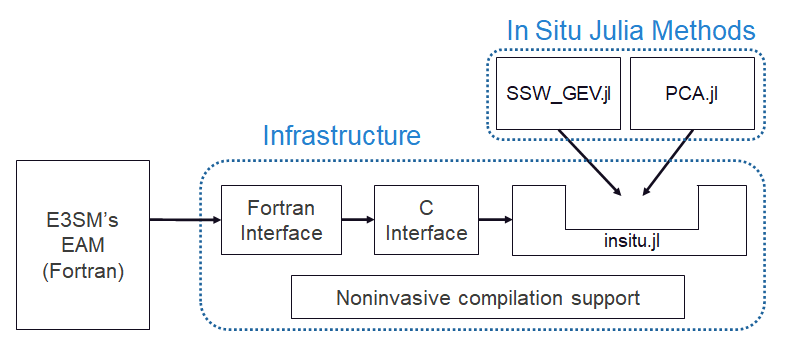
\includegraphics[width=\linewidth, height=3.5cm]{figures/infra.png}
    \caption{Overall infrastructure design.}
    \label{fig:infra}
\end{figure}



\subsection{Fortran Interface}



To couple E3SM's EAM with Julia, we implement a Fortran-based in situ interface in EAM to manage in situ Julia data analysis and pre-process the EAM simulation data. Specifically, this interface is implemented in EAM's \texttt{stepon} component, but we note this interface could be used for in situ data analysis on other E3SM components with minimal effort. Two major tasks are implemented in our Fortran interface. First, this interface calls the worker function of actual in situ Julia data analysis at every time step, and the initialization/cleanup functions at the first/last time step. Second, the interface wraps the EAM simulation data with its supportive data (e.g., data length, time step) and passes the pointer of the wrapped data to the C interface for removing explicit data copy. Also, this adapter passes an internal E3SM MPI communicator to the C interface. When the E3SM simulation is running at large-scale, each MPI rank of EAM calls its own Fortran interface and initiates one Julia instance. For the time steps between the first and last time step, each in situ Julia instance returns the control back to its parent EAM after it finishes its data analysis. After Julia returns its control back to EAM, the Julia runtime is still working and keeps global variables alive for usage in following time steps.



\subsection{C Interface}


The C interface stands between the Fortran and Julia interfaces, which aims to efficiently implement the functions in the Fortran interface for interacting with Julia. The C interface includes three major functions: initialization, cleanup, and worker, which creates an in situ Julia instance (by loading and initializing the in situ Julia module from a specified path), destroys the Julia instance, and passes the data from the Fortran interface to the in situ Julia instance (i.e., Julia interface). The following code snippet shows the major parts of the initialization and cleanup functions in the C interface.

\begin{minipage}{\linewidth}
\begin{lstlisting}[language = C, caption={C interface initialization and cleanup.}]
jl_function_t *f;
void jl_init_(){
  jl_init__threading();
  jl_eval_string("Base.include(Main, \
  \"insitu.jl\")");
  jl_eval_string("using Main.mymodule");
  jl_module_t *mod_name = \
  (jl_module_t*)jl_eval_string("Main.mymodule");
  f = jl_get_function(mod_name, "streaming");
  return ;
}
void jl_exit_(){
  jl_atexit_hook(0);
  return ;
}
\end{lstlisting}
\end{minipage}


The worker function in the C interface aims to support efficient low-level data communication between E3SM and the in situ Julia data analysis. The key implementation of this C interface is shown in the following code snippet. Each MPI rank of EAM has access to only a local data block of EAM variables (e.g., velocity and temperature) and passes its local data block's pointer (e.g., \texttt{arr} and \texttt{p\_arr} in the code snippet) to its own in situ Julia instance through the C interface. When the in situ Julia instance needs remote data (e.g., for computation of SSW) from other in situ Julia instances, \texttt{MPI.jl} is used in the Julia interface to implement the data communication between different in situ Julia instances. However, one key design challenge is to assure that E3SM and Julia use the same MPI communicator for correct data communication, as current Julia C embeddings are not able to directly pass the MPI communicator. To address this challenge, we transfer the original Fortran MPI communicator to this C interface without conversions, and then wrap it as \textit{jl\_box\_int32} and pass it to the Julia interface. The Fortran MPI communicator will be converted to Julia MPI communicator in the Julia interface. It is also important to conduct garbage collection (GC) in this C interface for every time step. This is because \texttt{arr} and \texttt{p\_arr} in the code snippet are allocated and then deallocated in E3SM for every time step, and the Julia runtime is not aware of this and hence needs explicit GC.

\begin{minipage}{\linewidth}
\begin{lstlisting}[language = C, caption={C interface worker.}]
void jl_worker_(double *arr, int* arrlen,  \
int* p_arr, int* p_len, MPI_Fint *Fcomm){
  jl_array_t *x = NULL, *y = NULL;
  jl_value_t *jl_comm = NULL;
  JL_GC_PUSH3(&x, &y, &jl_comm);
  x = jl_ptr_to_array_1d(jl_apply_array_type \
  ((jl_value_t*)jl_float64_type,1),arr,*arrlen,0);
  y = jl_ptr_to_array_1d(jl_apply_array_type \
  ((jl_value_t*)jl_int32_type,1),p_arr,*p_len,0);
  jl_comm = jl_box_int32(*Fcomm);
  jl_call3(f,(jl_value_t*)x,(jl_value_t*)y,jl_comm);
  JL_GC_POP();
  return ;
}

\end{lstlisting}
\end{minipage}



\subsection{Julia Interface}

The Julia interface mainly defines the format of input data, so all in situ Julia data analysis methods can be plugged-in without additional E3SM compilation, thanks to Julia's Just-in-time (JIT) compilation.
As discussed previously, another key design of the Julia interface is to correctly convert the Fortran MPI communicator to Julia MPI communicator, which enables the algorithm developers to write their analysis routines using the same EAM MPI communicator. Due to the low-level MPI implementations, different MPI libraries (i.e., OpenMPI, MPICH, and MVAPICH) require specific converters; the following code snippet shows the converter implementations~\cite{gabriel2004open,panda2013mvapich,gropp1996user}.

\begin{minipage}{\linewidth}
\begin{lstlisting}[language = Julia, caption={Juila interface MPI conversion.}]
\\ OpenMPI
Jcomm = MPI.Comm(ccall((:MPI_Comm_f2c, \
        "openmpi/lib/libmpi.so"),Ptr{Cvoid}, \
        (Cint,),Cint(Jcomm)))

\\ MPICH and MVAPICH
Jcomm = MPI.Comm(Cint(Jcomm))
\end{lstlisting}
\end{minipage}


\subsection{Noninvasive Compilation}
The final design consideration is the compilation and execution design of coupling Julia with E3SM. The Fortran interface is implemented inside EAM, and the C interface file is placed in the same folder of the Fortran interface. The in situ Julia module is placed in the same run folder with the E3SM executable. As E3SM mixes the usage of GNU Make and CMake for combining and compiling different E3SM components, we have added the Julia compilation flags for the C and Fortran interfaces into the EAM CMake file (i.e., header files) and the top-level GNU Make file (i.e., Julia libraries). The in situ Julia module is only compiled when it is called during runtime, which avoids recompiling the whole of E3SM if the in situ Julia module needs to be changed.





\section{Data Analysis Modules}
In this section, we describe the two demonstration data analysis modules: detecting SSW with extreme value modeling, and TributaryPCA.

\subsection{Sudden Stratospheric Warming (SSW)}
Our first in situ climate analysis algorithm detects extreme weather events called SSWs. By definition, SSW is characterized as a major midwinter warming that occurs when the daily zonal mean zonal winds at $60^{\circ}$N and $10$ hPa (hectopascal) become easterly for at least $10$ consecutive days between November and March~\cite{ssw,ssw_def}. This event can result in extremely cold temperatures at Earth's surface, causing hazardous weather and disrupting many socioeconomic sectors. Since the robust detection of rare SSW events requires spatiotemporal climate data at high temporal frequencies, for high-resolution EAM runs, post-hoc SSW detection capabilities are limited as storage of high-resolution and high-frequency climate data would be prohibitive. Therefore, an in situ SSW detection algorithm is required.

Here, we briefly present the distributed SSW detection technique that we have developed and deployed in situ with EAM. During the simulation run, when a time marks the end of a day, we further process data from that time step. Initially, we compute the the zonal mean zonal wind at each MPI process independently using zonal velocity (U-velocity). As the EAM mesh does not put grid points exactly at $60^{\circ}$N and $10$ hPa, we first filter two layers of grid points, which are above and below the $10$ hPA pressure level and fall within [$59^{\circ}$N - $61^{\circ}$N] at each MPI process. Then, we linearly interpolate the zonal wind values to obtain values at $60^{\circ}$N and $10$ hPa. Then, using an MPI reduction, we estimate the final global daily zonal mean zonal wind value. Based on the definition of SSW, this value needs to be negative for $10$ consecutive days, so we maintain a global counter variable that keeps track of the number of consecutive days for which the value is negative. Once the value of that counter reaches $10$, we record a SSW event for that simulation year. A pseudo code for this algorithm is provided in Algorithm~\ref{ssw_algo}. Note that when a SSW event is detected, the climate scientists typically are interested in collecting more data from following time steps, so the SSW detection can be used as a triggering event. Using SSW as a triggering event can reduce the overall in situ computation load since the SSW-specific analyses will only happen adaptively when a SSW event is detected.



To characterize spatial patterns in surface temperature across CONUS following a detected SSW (compared to no detected SSW), we fit two separate GEV models, similar to~\cite{ssw_isav}. These models represent the distribution of the daily minimum temperatures. Specifically, we transform the surface temperature data by subtracting 300$^\circ$K and multiplying by negative one, then fit GEV models. As described in~\cite{ssw_isav}, Algorithm 1, model parameters are updated periodically using a buffer of recent data, depending on whether or not an SSW event was recently detected. In this paper, we update the GEV models every three days, using the last three days of daily minimum temperatures as the data for modeling. The fitted GEV models then represent distributional information about the data through their parameter estimates, which are updated in situ without the need to save the raw data. In this work, each time the GEV models were to be updated, we used 10 Monte Carlo samples in evaluating each gradient and 500 total optimization iterations each time the models were updated. We used the Adam optimizer from Turing~\cite{ge2018turing} with a learning rate of 0.0001. 

\subsection{TributaryPCA} 
As described more fully in~\cite{wang2021tributarypca}, TributaryPCA solves the standard PCA objective in a distributed, online fashion; we give a brief overview of the implementation here.
Let $X \in \mathbb{R}^{d \times N}$ be a data set consisting of $N$ samples with unknown covariance $\Sigma \in \mathbb{R}^{d \times d}$. 
In our application, $N$ is the number of time points and $d$ is the number of spatial locations.
PCA seeks a $k$-dimensional orthonormal subspace $V \in \mathbb{R}^{d \times k}$ such that when the data are projected onto $V$, their variance is maximized. This amounts to solving 
\begin{equation}\label{eqn:pca-obj}
    \max_{\substack{V \in \mathbb{R}^{d \times k} \\ V^TV = I_k}} \text{Tr}\Big(V^T \Sigma V\Big).
\end{equation}
Equation~\eqref{eqn:pca-obj} is maximized by the top-$k$ eigenvectors of $\Sigma$, so the classical PCA calculation computes the top-$k$ eigenvectors of the estimated covariance matrix.
However, this approach is not feasible when data arrives sequentially (so that all $N$ samples are not available at one time) or when the dimension of the data is large (so that it is not stored centrally on one compute node).
In the streaming setting, the AdaOja algorithm~\cite{henriksen2019adaoja} seeks to estimate the solution to Equation~\eqref{eqn:pca-obj} using projected stochastic gradient descent with an automatically-tuned step size.
That is, the estimated eigenvectors $V$ are adjusted as each data point arrives (over time) using the gradient of Equation~\eqref{eqn:pca-obj} evaluated at the new data point.
This procedure consists of three key steps: a gradient computation, a learning rate update, and a QR decomposition (to ensure orthogonality of the estimated eigenvectors).
The TributaryPCA algorithm (1) computes the gradient in a distributed fashion using data stored on each node and MPI \texttt{allreduce}, (2) updates the learning rate in a distributed fashion using MPI \texttt{allreduce}, (3) applies the stochastic gradient update on each node, and (4) uses distributed linear algebra~\cite{demmel2012communication} to orthogonalize the estimated $V$ (collected from all nodes using MPI \texttt{reduce}).
The key portion of the in situ code (that would be called at each time step during the simulation) is shown in the following listing, where \texttt{X\_par} is the data on the current node, \texttt{V\_par} is the node's spatial subset of the current global estimate of the eigenvectors, \texttt{comm} is the MPI communicator object, \texttt{master} denotes the root/master node, and \texttt{grad\_par}, \texttt{abs2}, $\alpha$ are pre-initialized arrays.


\begin{minipage}{\linewidth}
\begin{lstlisting}[language = Julia, caption={Key algorithmic steps of TributaryPCA in Julia.}]
# Compute gradient
XT_V_par = copy(X_par') * V_par
XT_V = MPI.Allreduce(XT_V_par, +, comm)
mul!(grad_par, X_par, XT_V, 1.0/N, 0.0)
# Update learning rate α
s = sum(abs2, grad_par, dims = 1)[:]
grad_norm_sq = MPI.Allreduce(s, +, comm) 
α .+= grad_norm_sq 
# Apply local gradient update
α_r = reshape(sqrt.(α), (1, size(α, 1)))
V_par .+= grad_par ./ α_r
# Orthogonalize to form global update of V
VT_V_par = copy(V_par') * V_par
VT_V = MPI.Reduce(VT_V_par, +, master, comm)
if node_id == master
    chol = cholesky!((VT_V + copy(VT_V')) / 2)
    Rinv = inv(chol.U)
else
    Rinv = nothing
end
Rinv = MPI.bcast(Rinv, master, comm)
V_par .= V_par * Rinv
\end{lstlisting}
\end{minipage}





\section{Experiments}

This section first summarizes the experimental setup for our in situ tests, including the application setup, conducted problems, build process and the underlying systems. Then we will show the in situ data analysis results of our in situ SSW and PCA Julia modules. Finally, we discuss the performance of this framework and some insights of conducting in situ Julia data analysis with large-scale scientific applications on modern supercomputers.


\subsection{Setup}

We have run all our experiments on a cluster, Grizzly, located at Los Alamos National Laboratory (LANL). Grizzly consists of 1,490 compute nodes, and each node is equipped with two Intel Broadwell Xeon E5-2695v4 2.1GHz processors (18 cores per CPU) and 128GB 2400 MHz DDR4 memory.
The system runs on a Tri-Lab Operating System Stack (TOSS) and its nodes are connected by Intel OmniPath Host Fabric Interface (HFI) single port via PCIex16.
Grizzly uses Slurm for job scheduling and resource management. The total storage is 15PB.

To deploy our in situ algorithms, we have run the fully coupled E3SM simulation and accessed the data from its Atmosphere model, EAM, for analyses. The EAM module runs in conjunction with other coupled modules (MPAS-Ocean, MPAS Sea Ice, MPAS Land Ice, and Land Surface) to produce scientifically meaningful climate data. In this work, we use a realization of the Shared Socioeconomic Pathway (SSP) $585$ scenario~\cite{Eyring} with E3SM. This is an aggressive scenario that assumes the climate will experience an increase in radiative forcing of $8.5$ W/m$^2$. We use the standard E3SM V1 configuration with a $1^{\circ}$ atmosphere and land (equivalent to 110 km at the equator), $0.5^{\circ}$ river model ($55$ km), and an ocean and sea ice with mesh spacing varying between $60$ km in the midlatitudes and $30$ km at the equator and poles~\cite{e3sm_v1}. %To run optimally, E3SM simulation test cases are often configured to run on a specific number of MPI processes and this particular case is optimized to run on $3024$ cores, which is equivalent to running it on $84$ computing nodes in Grizzly.


Our tests fall into two data analysis tasks: SSW and PCA. Importantly, E3SM is only compiled once, and we can then switch between the PCA and SSW in situ Julia modules. The Julia modules are dynamically compiled and executed by using the Julia $1.8$ version. Each in situ run is performed 10 times to mitigate system noise. We also add timers in the slurm system for measuring performance and overhead.

\subsection{In Situ SSW Detection and Characterization Results}
After running for 365 simulation days (one simulated year), with the GEV models updated every three days, we found that the post-SSW GEV model was updated 11 total times while the non-SSW GEV model was updated 110 times.
More detailed analysis of offline data, including comparison of SSW and non-SSW models, can be found in~\cite{ssw_isav}; for the purposes of this paper, we will show the GEV modeling results for the non-SSW simulation periods because the models were updated more total times.
Figure \ref{fig:ssw_results} shows the GEV model parameters $\mu$ (location) and $\beta$ (scale) for the non-SSW time periods at the conclusion of one simulated year. 
While the parameter values can be somewhat difficult to interpret directly, we emphasize that these saved parameter values, taking only a fraction of the storage space of the original data, can provide rich information about the distribution of minimum temperatures; for instance, we can use the model parameters to answer questions such as ``What is the probability that the minimum temperature is more than 10 degrees Kelvin lower than the average value?''
In this relatively short simulation run, we see that the spatial patterns in the parameter plots are somewhat rough and non-smooth, particularly for $\beta$; we expect that longer simulation runs and modifications to the GEV variational inference scheme could improve our estimates. 
However, it is promising that some noticeable spatial structure appears; for example, both $\mu$ and $\beta$ appear to be smaller over the Atlantic Ocean, mirroring the tendency of temperatures to be more stable over the ocean (less fluctuation in the minimum value). 
We take these results as a promising sign that our models can capture relevant information, though due to the relatively short simulation time period, we leave making any claims based on these models for future work.

\begin{figure}
    \centering
    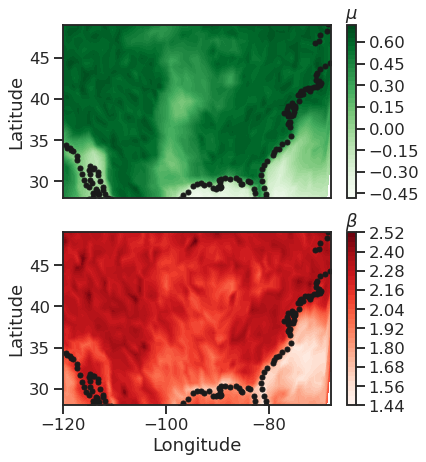
\includegraphics[width=0.8\linewidth]{figures/ssw_results.png}
    \caption{Generalized extreme value (GEV) model parameter estimates at the end of one simulation year for the non-SSW time periods across the continental United States (coast line denoted with black points). Top: location parameter $\mu$, which shows notable spatial patterns over the Atlantic Ocean and Gulf of Mexico; in addition, a band of lower $\mu$ values appears to stretch through the Midwest region. Bottom: scale parameter $\beta$, which has less smooth spatial structure, but some similarities to the top figure in terms of lower values over bodies of water and through the Midwest region.}
    \label{fig:ssw_results}
\end{figure}

\subsection{PCA Results}
Over the one-year simulation run, we extracted the top three spatial principal components of the surface temperature variable using the TributaryPCA method.
Figure \ref{fig:pca_results} shows spatial plots of these three principal components. 
Each component indicates a different spatial pattern of warming (red color) and cooling (blue color) extracted from the simulation data.
In particular, the first component indicates cooler temperatures away from the equator. 
The second component indicates warming across much of the Eastern hemisphere, with cooling in the Americas and parts of Africa. 
The third component indicates cooling in Africa and Europe with warming elsewhere.
While these components were extracted from a fairly short simulation run, the results demonstrate the ability of TributaryPCA to extract important climate patterns while running in a distributed in situ environment, without saving any raw data for post-processing.
\begin{figure}
    \centering
    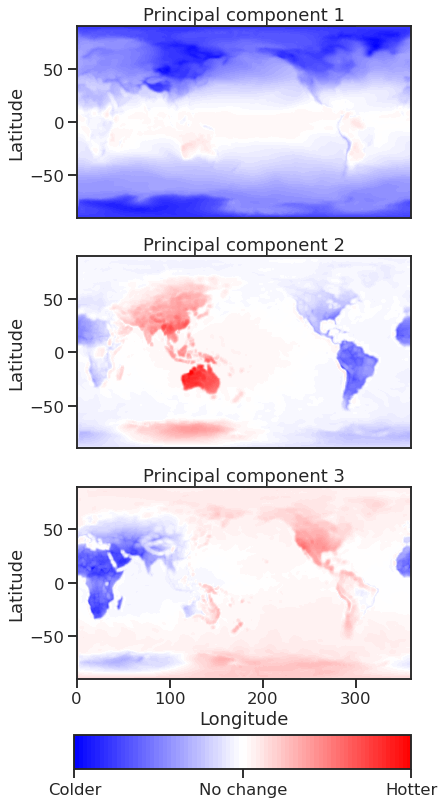
\includegraphics[width=0.8\linewidth]{figures/insitu_pca.png}
    \caption{First three spatial principal components obtained by in situ TributaryPCA method. Within each component, white color indicates no change to surface temperature, while blue indicates colder and red indicates hotter temperatures. The first principal component appears to indicate mild tropical warming with cooling away from the equator. The second principal component indicates warming in much of the Eastern hemisphere and cooling in Africa and the Americas, while the third component indicates primarily cooling in Africa and Europe.}
    \label{fig:pca_results}
\end{figure}

\subsection{Performance}

This section studies the performance of our developed in situ framework and how the framework impacts the performance of E3SM. Based on these studies, we will make suggestions for integrating in situ Julia analysis with large-scale HPC applications.

\subsubsection{Problem and Processing Element (PE) Layout}\hspace*{\fill} \\


The atmosphere component of E3SM, CAM, uses a spectral element dynamical core at 110-km resolution on a cubed sphere geometry. It has 72 layers with a top at approximately 60 km. The main atmosphere physics time step is 30 minutes and the ne30 grid used as the E3SM v1 main configuration has 5400 horizontal elements. So, we define nine different PE layouts in Table~\ref{table:layout} to distribute the workload of 5400 atmospheric elements evenly (for performance evaluation), as well as the other components. Some of the other components run sequentially with CAM, using the same processors as it does, while other run concurrently on a different set of processors. 




\begin{table}
  \caption{PE Layout}
  \label{table:layout}
  \begin{tabular}{ccl}
 \toprule
 PE Layout& Number of PEs & Number of PEs per node\\
 \midrule
 100\%S & 1350 & 36 \\
 50\%S  & 1350 & 18\\
 25\%S  & 1350 & 9\\
 100\%M & 1800 & 36\\
 50\%M  & 1800 & 18\\
 25\%M  & 1800 & 9\\
 100\%L & 2700 & 36\\
 50\%L  & 2700 & 18\\
 25\%L  & 2700 & 9\\
 \bottomrule
\end{tabular}
\end{table}


\subsubsection{Framework Performance}\hspace*{\fill} \\

We first run the high-resolution E3SM problem with both of the SSW\_GEV and PCA in situ analyses. For each analysis, we run with the predefined nine different PE layouts. Figures \ref{fig:ssw_break} and \ref{fig:pca_break} show the execution time breakdown for the SSW\_GEV and PCA in situ experiments, respectively. The blue bars represent the ratios of analysis execution time to the total EAM execution time. The overhead execution time includes the data preparation for the Julia module, loading Julia module, and clean up the Julia module. It can be seen from the results that our developed SSW\_GEV only consumes less than 4\% of the total EAM execution time. PCA is more computationally intensive than SSW\_GEV, and it can take up to 26\% of the total EAM execution time. This is because the main tasks of SSW\_GEV and PCA are linear interpolation and Cholesky decomposition, respectively, with the latter being considerably more complex to compute. In addition, it can be observed that the in situ analysis consumes more time of the EAM execution time for larger layouts and higher PE usage on each node. This is because EAM generates less data per node in large layouts and the in situ analysis is less performance-sensitive than EAM in terms of data reduction. Also, higher PE usage per node raises memory pressure for the in situ analysis.

\begin{figure}
    \centering
    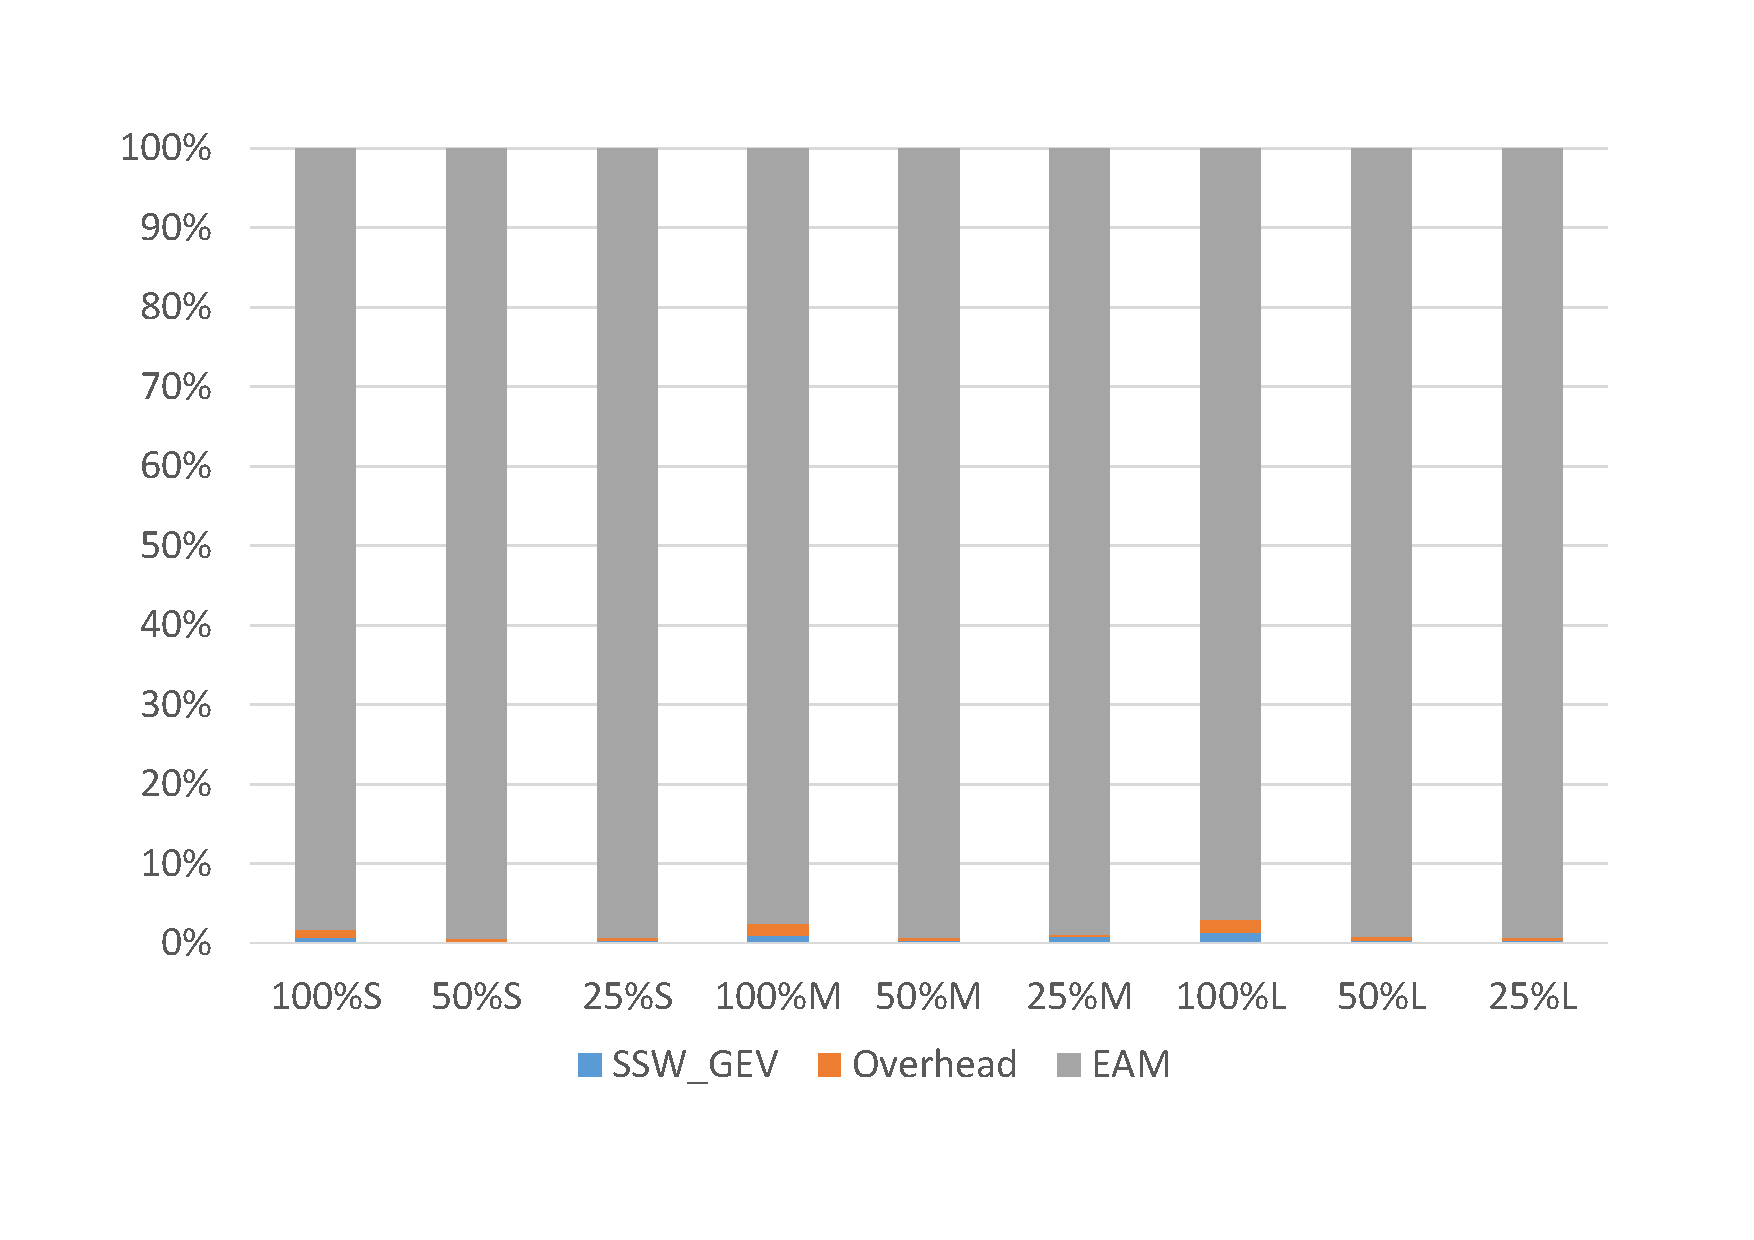
\includegraphics[width=\linewidth, height=5.5cm]{figures/ssw_break.pdf}
    \caption{Execution time breakdown for the SSW\_GEV in situ analysis.}
    \label{fig:ssw_break}
\end{figure}


\begin{figure}
    \centering
    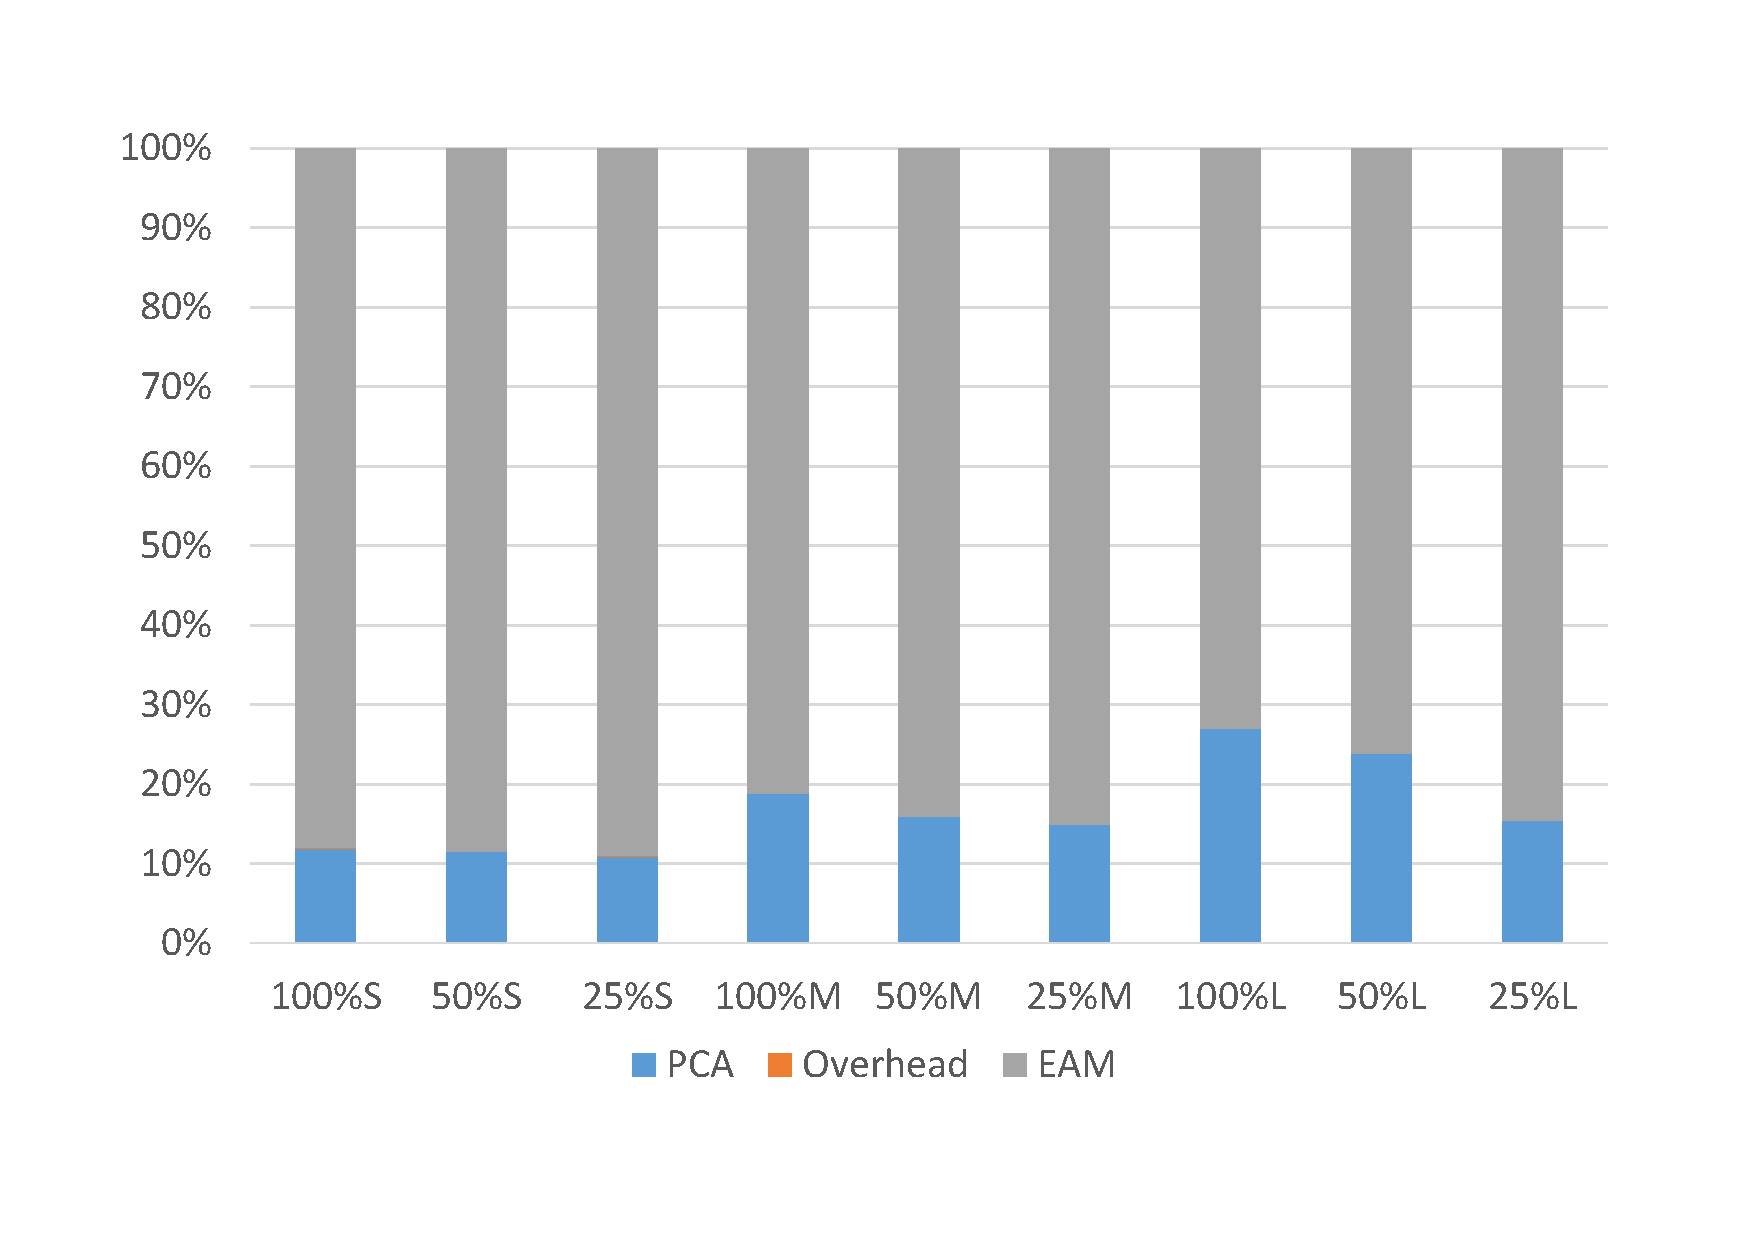
\includegraphics[width=\linewidth, height=5.5cm]{figures/pca_break.pdf}
    \caption{Execution time breakdown for the PCA in situ analysis.}
    \label{fig:pca_break}
\end{figure}



\subsubsection{E3SM performance trends}\hspace*{\fill} \\

To study how the in situ analysis impacts the E3SM performance, we also run the original E3SM without the in situ framework. Figures \ref{fig:ssw_trend} and \ref{fig:pca_trend} show the performance trends of the EAM components with different PE layouts for the SSW\_GEV and PCA in situ experiments, respectively. As discussed in the previous section, SSW\_GEV is lightweight and its performance trend is flat comparing to the EAM component. Also, the EAM component itself is almost not impacted by the in situ framework. The only exception is the high PE usage per node and the reason is limited memory shared by E3SM and the Julia runtime and module. For PCA, the only performance overhead of the in situ framework is from the Julia analysis, where high PE usage per node can cause up to 6\% additional overhead for SSW\_GEV with the 100\%L layout. 


\begin{figure}
    \centering
    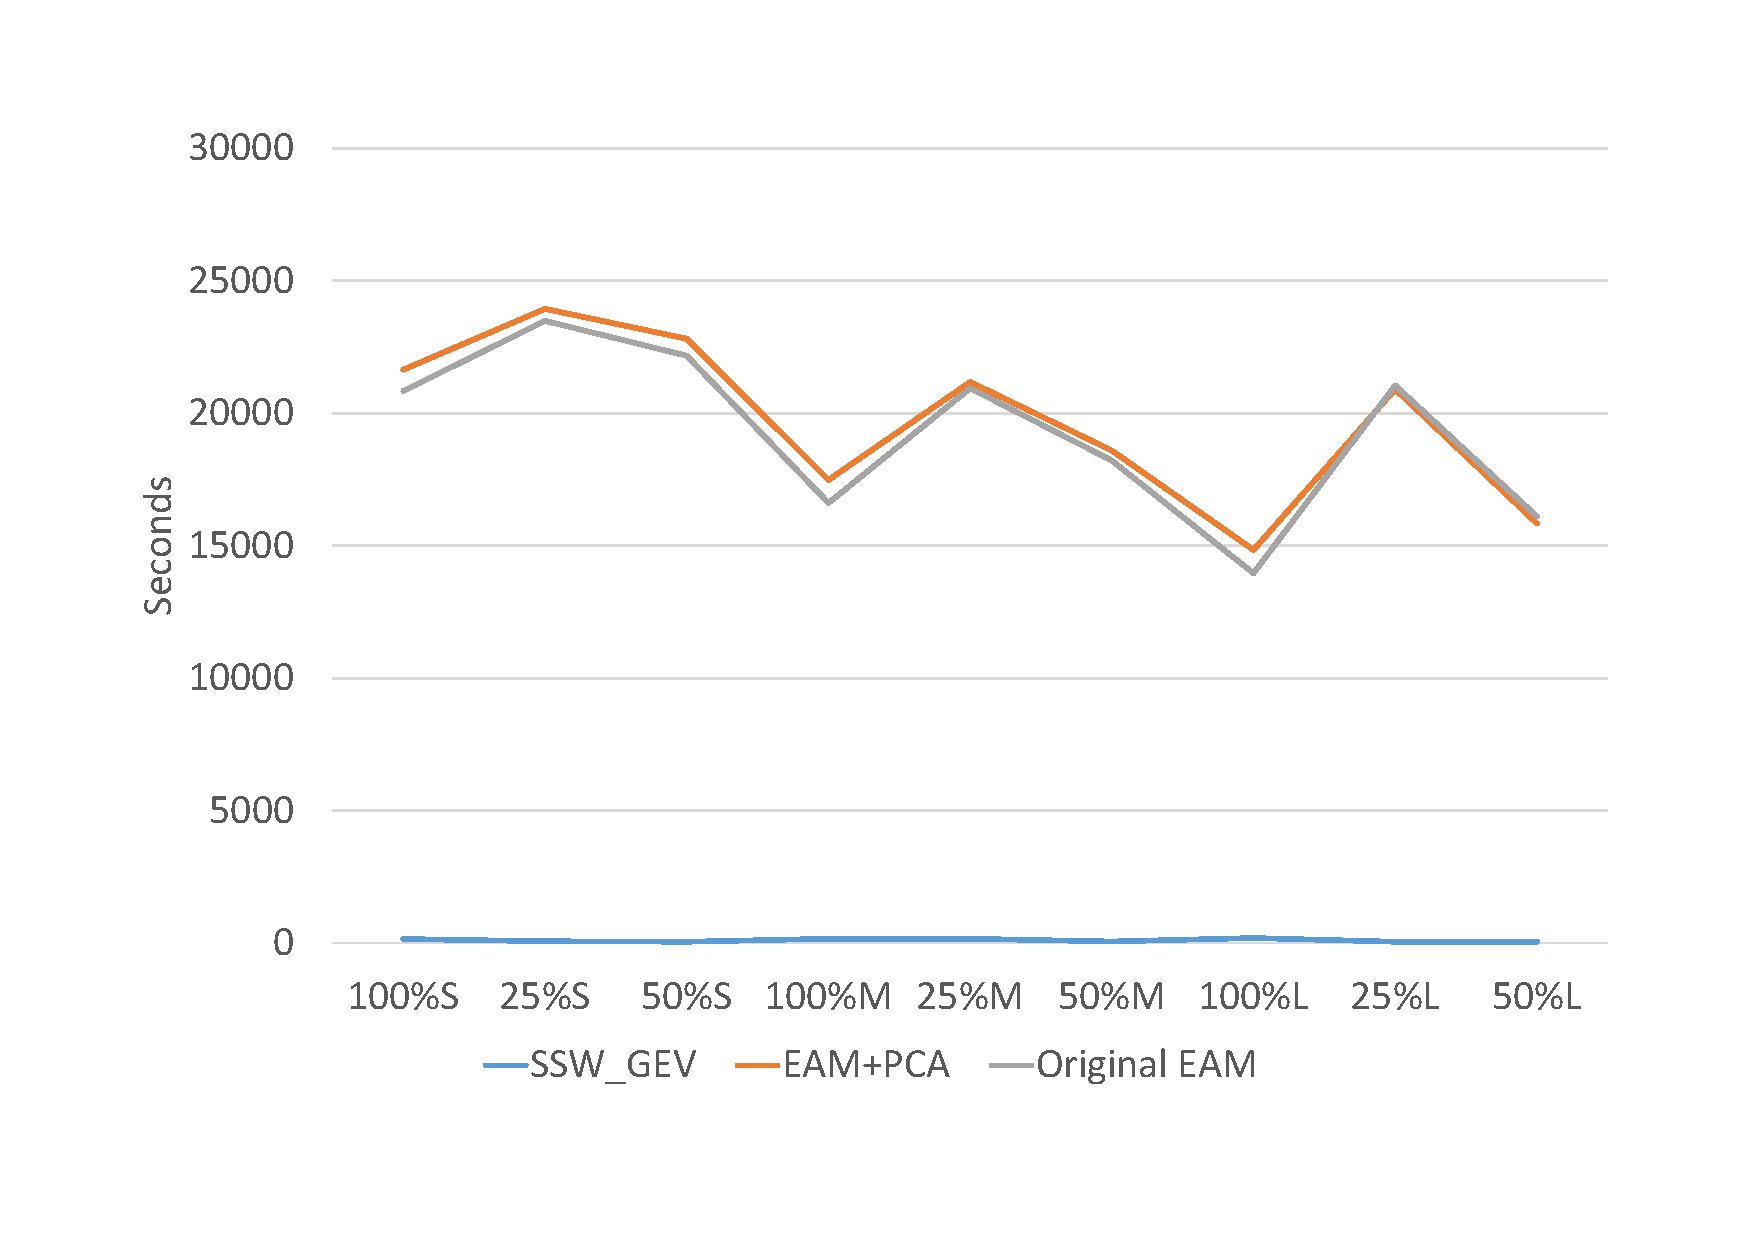
\includegraphics[width=\linewidth, height=5.5cm]{figures/ssw_trend.pdf}
    \caption{Execution time trends of the SSW\_GEV in situ analysis and the EAM component.}
    \label{fig:ssw_trend}
\end{figure}


\begin{figure}
    \centering
    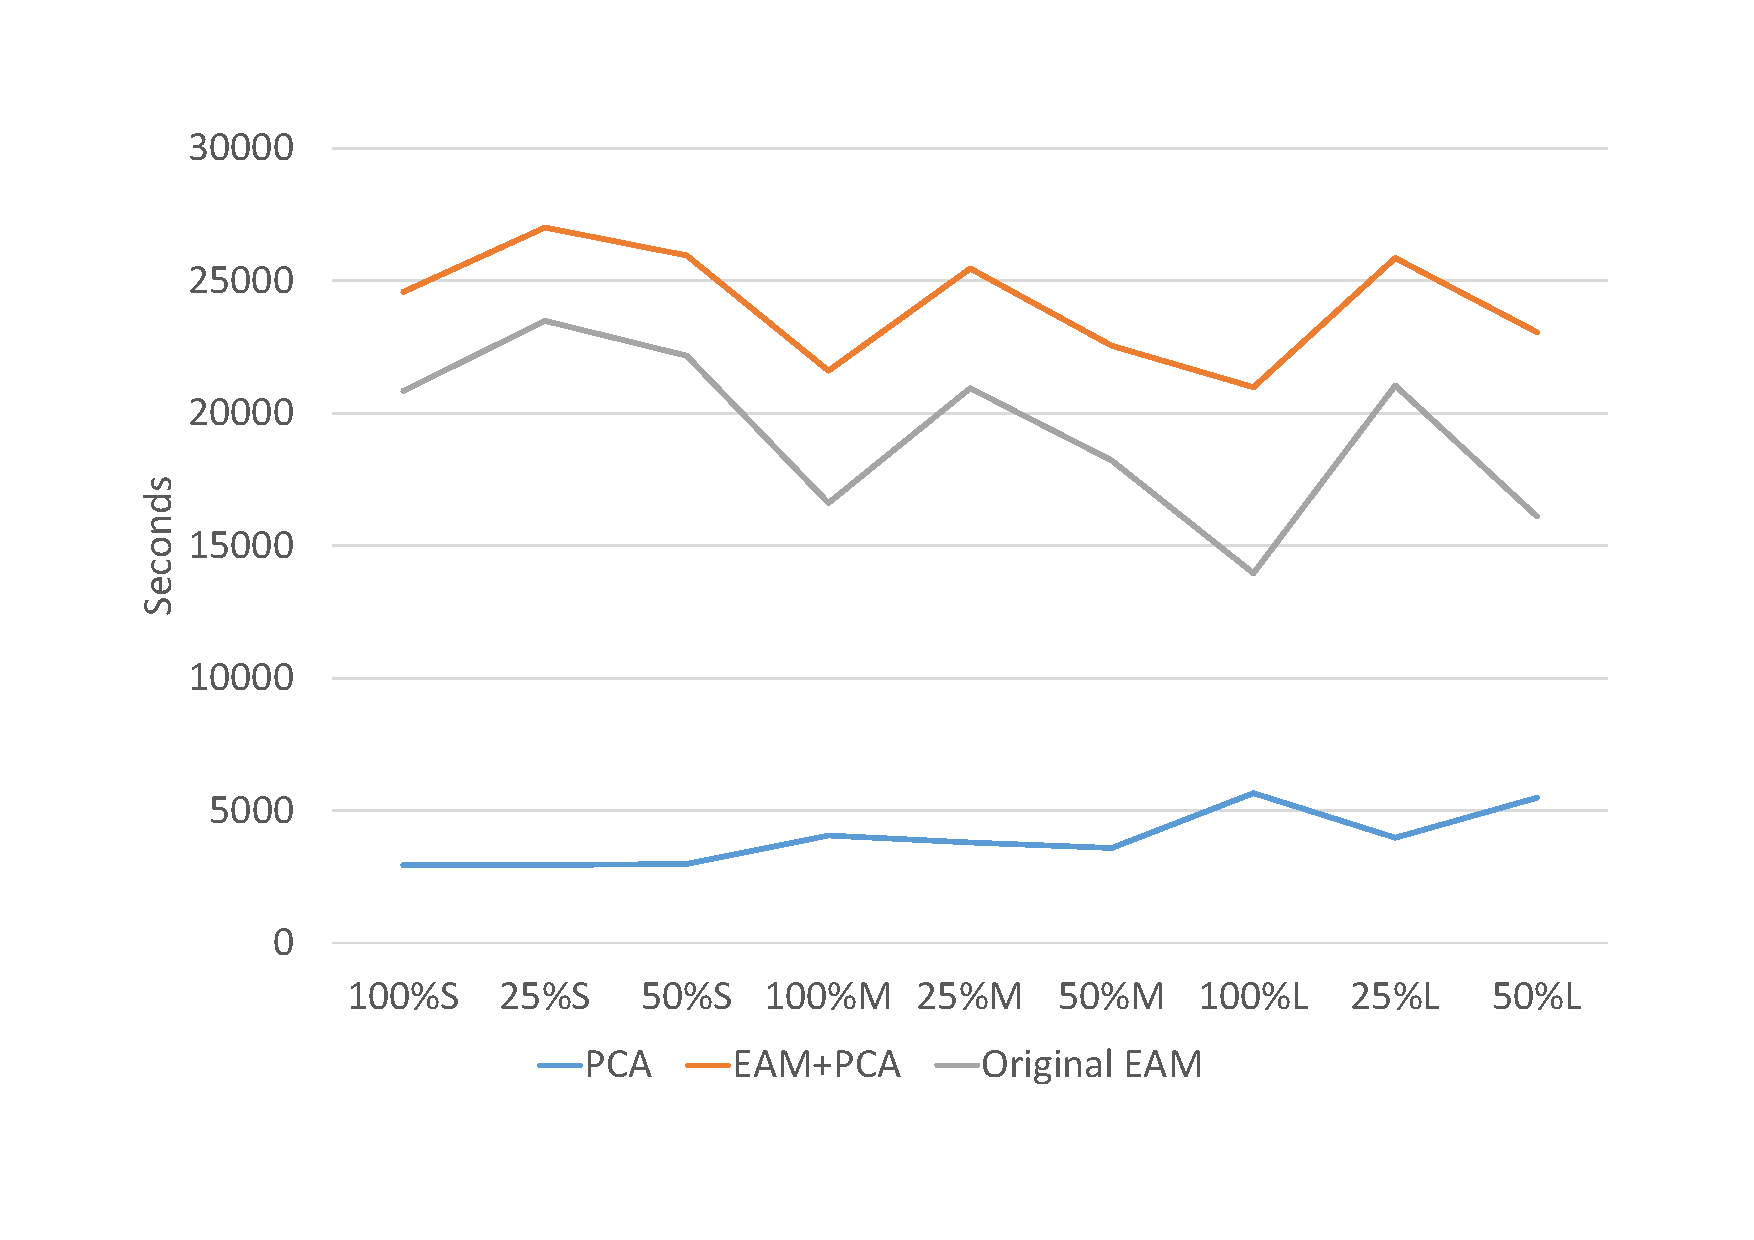
\includegraphics[width=\linewidth, height=5.5cm]{figures/pca_trend.pdf}
    \caption{Execution time trends of the PCA in situ analysis and the EAM component.}
    \label{fig:pca_trend}
\end{figure}


\subsubsection{Performance variations across MPI ranks}\hspace*{\fill} \\

We examine the performance variations across all MPI ranks for SSW\_GEV and PCA in this section. As we run the same high-resolution problem for 12 months for all of our experiments, the load balancing is only impacted the total number of PEs (i.e., S, M, and L). Figures \ref{fig:ssw_outliers} and \ref{fig:pca_outliers} show the performance variation results for the SSW\_GEV and PCA in situ experiments, respectively. The performance is represented by processing rate, which is defined as the number of single-precision floating point variables that can be processed in one second. The blue, orange, and grey bars represent the slowest, average, and fastest processing rates. First, it can be seen from the figures that SSW\_GEV has higher variation than PCA, and this is due to the root PE of SSW\_GEV being responsible for data collection. Second, medium PE usage (i.e., 50\%) per node achieves a balanced combination of low performance variations and higher average processing rate. 

\begin{figure}
    \centering
    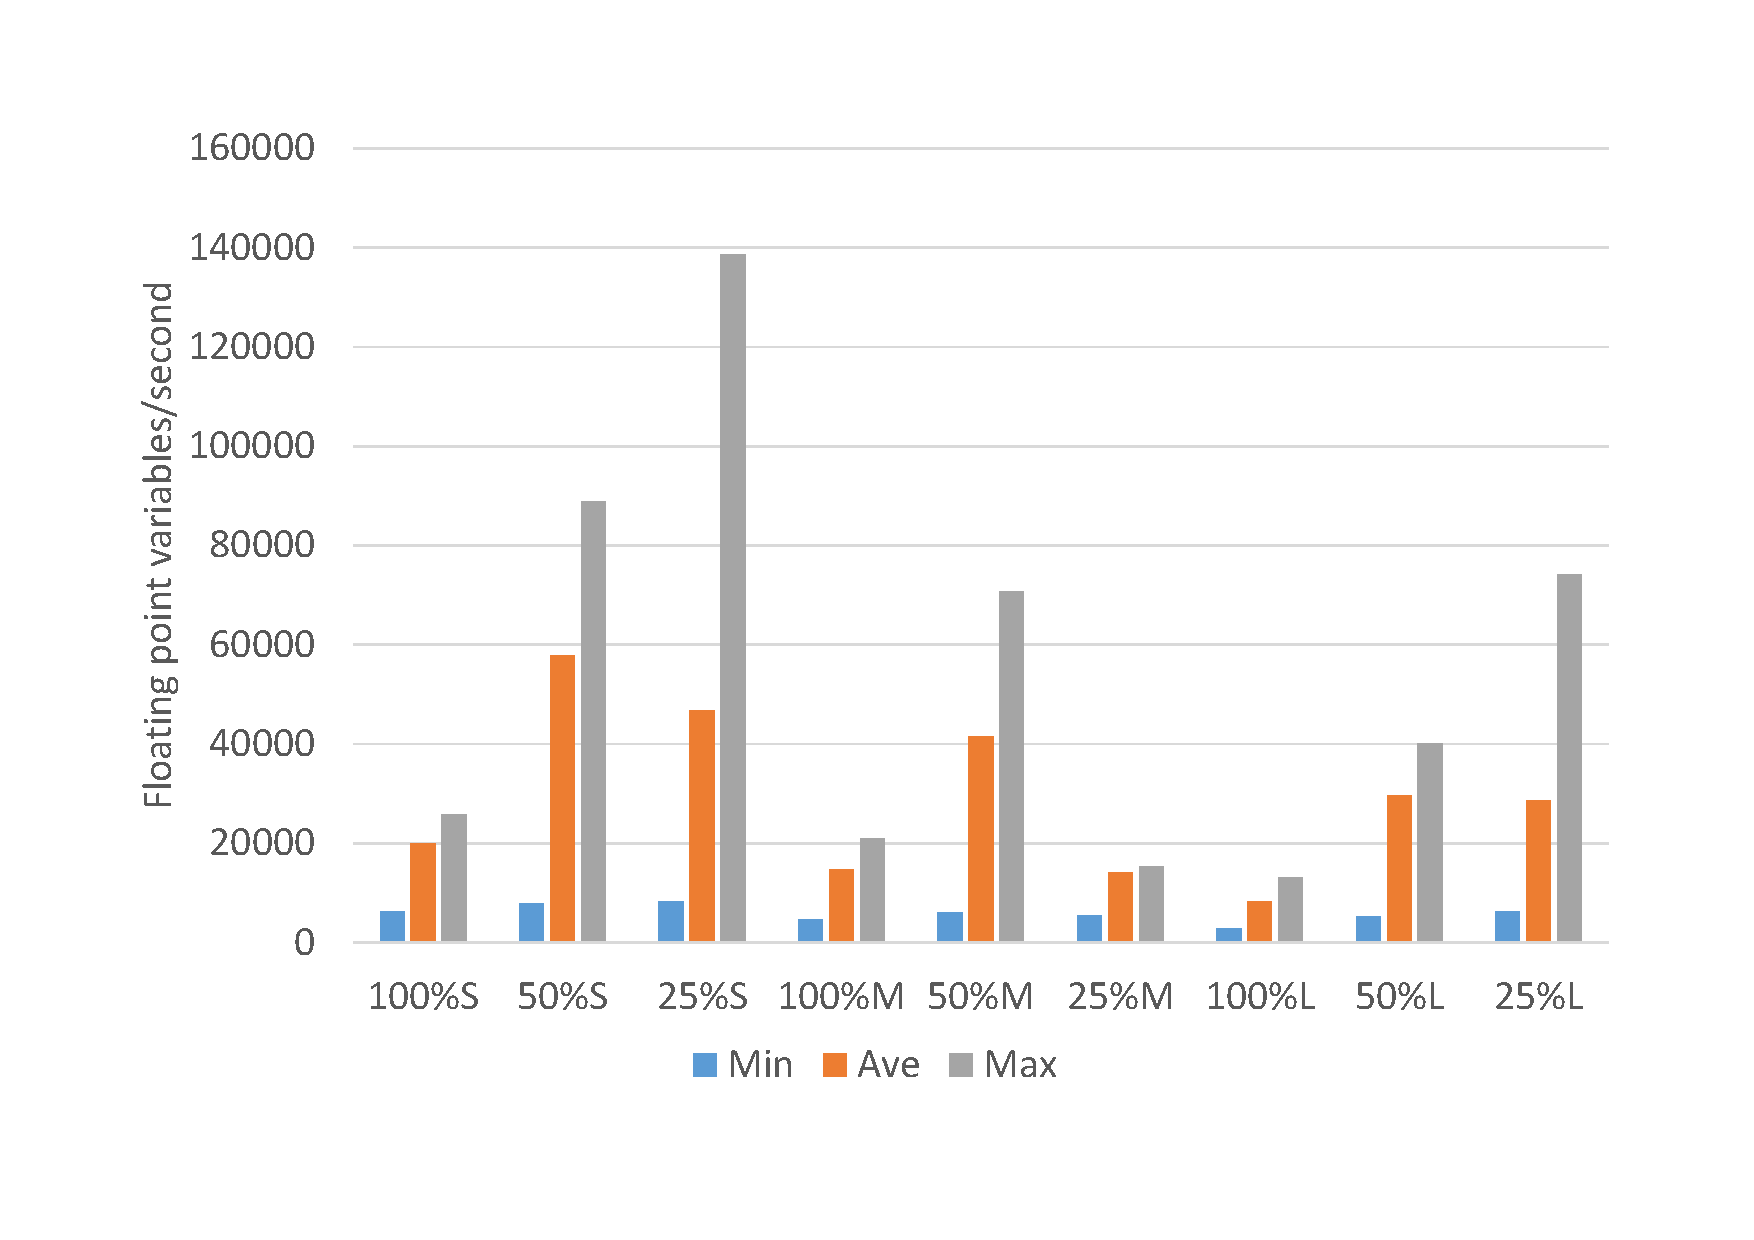
\includegraphics[width=\linewidth, height=6cm]{figures/ssw_outliers.pdf}
    \caption{Execution time of MPI ranks for the SSW\_GEV in situ analysis.}
    \label{fig:ssw_outliers}
\end{figure}


\begin{figure}
    \centering
    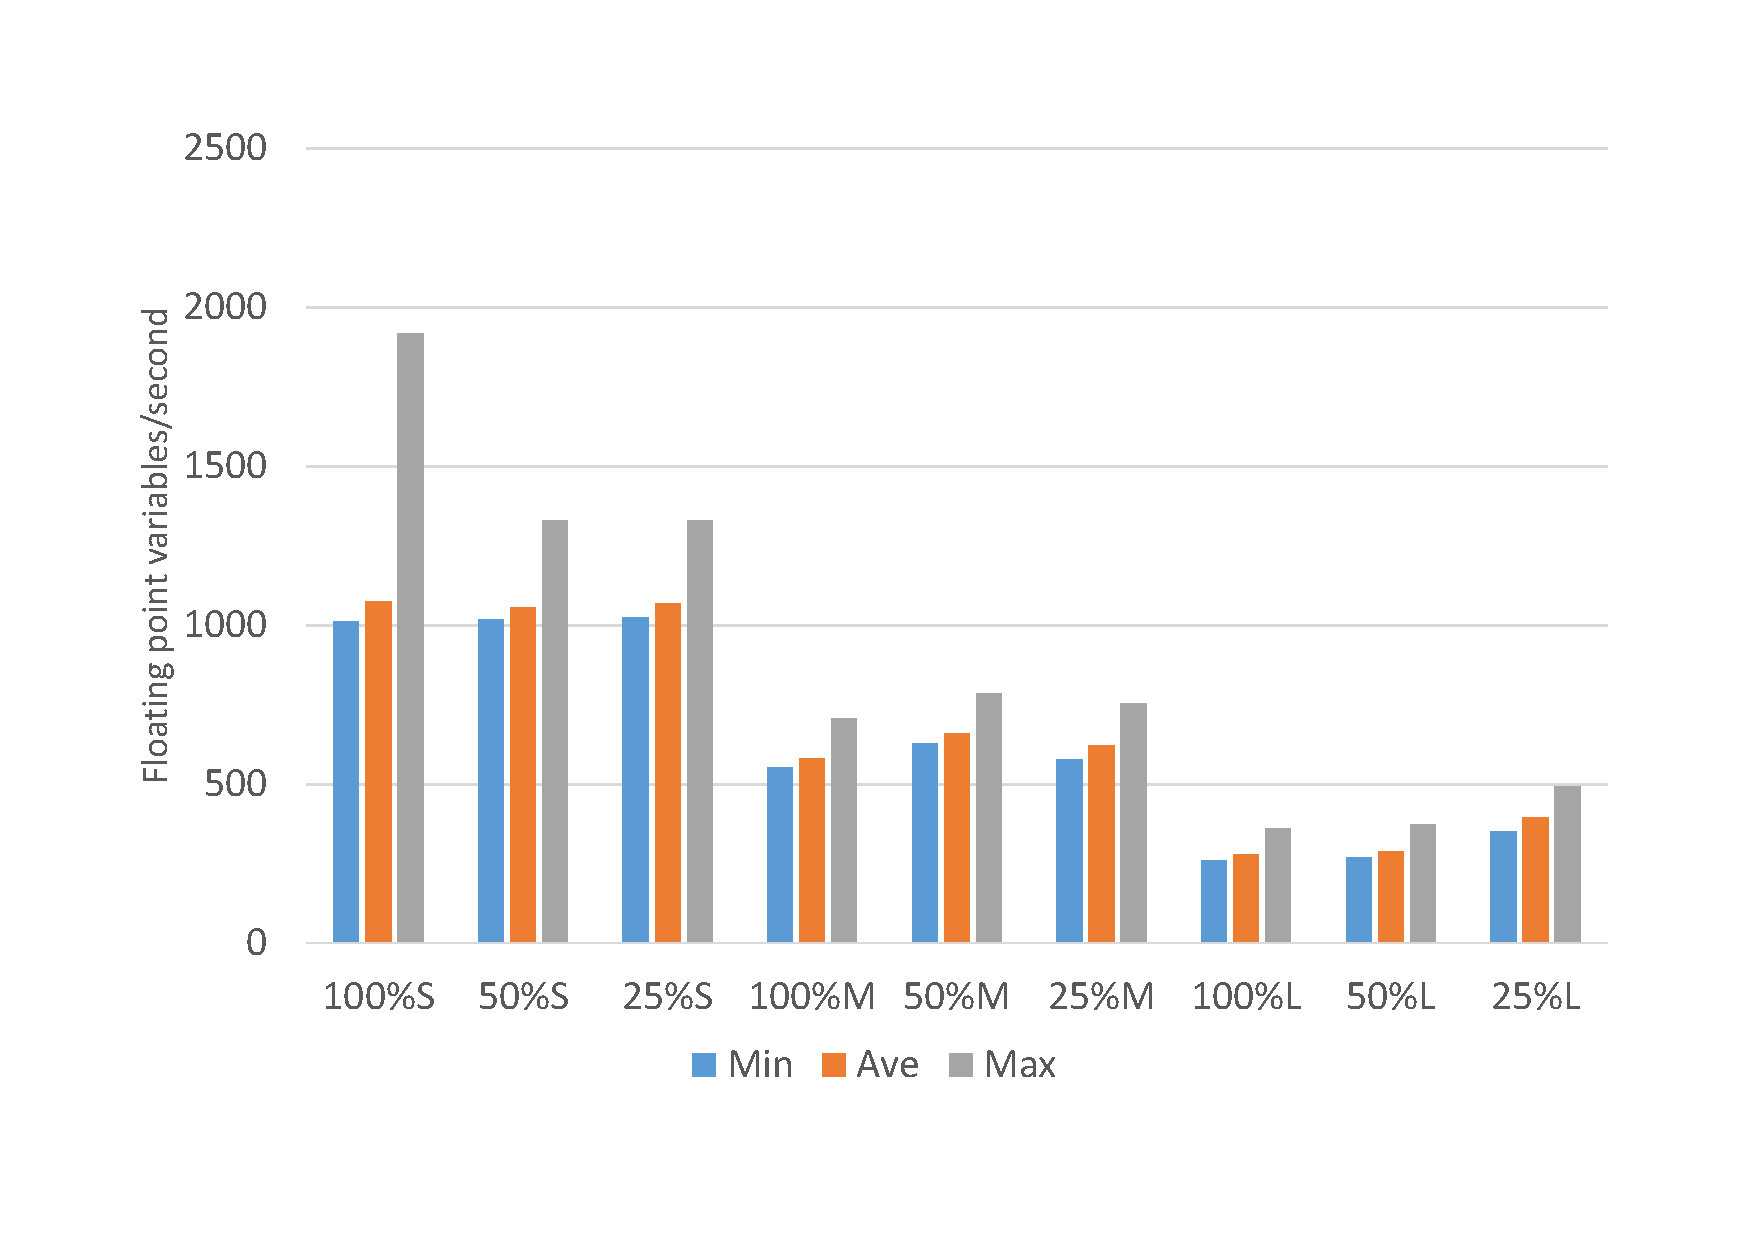
\includegraphics[width=\linewidth, height=6cm]{figures/pca_outliers.pdf}
    \caption{Execution time of MPI ranks for the PCA in situ analysis.}
    \label{fig:pca_outliers}
\end{figure}







\section{Conclusion}



This paper proposes a novel in situ infrastructure for coupling Julia with HPC applications and presents a practical case study of applying two in situ Julia data analysis methods to atmosphere data for detecting extreme weather events and characterizing climate patterns. The data presented in this paper suggest five high-level takeaway messages: (1)~the in situ infrastructure of coupling Julia with E3SM has insignificant overhead; (2)~our developed SSW\_GEV and PCA in situ modules in Julia are able to detect extreme weather events and characterize climate patterns with less than 26\% of total module execution time; (3)~a key performance factor of applying this in situ infrastructure is the total memory usage or pressure per node; (4)~the development of this in situ infrastructure and consqeuent Julia data analysis modules can be highly independent; (5)~future in situ Julia data analysis modules could be plugged-in without recompiling the whole HPC application. Having a comprehensive case study on this in situ infrastructure with production-level HPC application leads to a better support to our future efforts on applying advanced data analysis methods to existing HPC applications.


\section*{Acknowledgement}


Research presented in this paper was supported by the Laboratory
Directed Research and Development program of Los Alamos National
Laboratory under project number 20200065DR and is released
under LA-UR-22-31718. E3SM was obtained from the Energy Exascale
Earth System Model project, sponsored by the U.S.Department
of Energy, Office of Science, Office of Biological and Environmental
Research. This research used resources provided by the Los Alamos
National Laboratory Institutional Computing Program, which is
supported by the U.S. Department of Energy National Nuclear Security
Administration under Contract No. 89233218CNA000001.


% **************GENERATED FILE, DO NOT EDIT**************

\bibliographystyle{juliacon}
\bibliography{ref.bib}


\end{document}

% Inspired by the International Journal of Computer Applications template
